
\documentclass{standalone}
\usepackage{verbatim}
%
 \usepackage{lmodern}			% Usa a fonte Latin Modern		
\usepackage[T1]{fontenc}		% seleção de códigos de fonte.
\usepackage[utf8]{inputenc}		% determina a codificação utiizada (conversão automática dos acentos)
 \usepackage{helvet} %importando fonte helvet/arial equivalente
\usepackage{tikz}
\usetikzlibrary{arrows.meta,
                calc, chains,
                quotes,
                positioning,
                snakes,
                shapes.geometric}
% ------------------------------------------------------
 
% ------------------------------------------------------ 
\begin{document}
\pagestyle{empty}
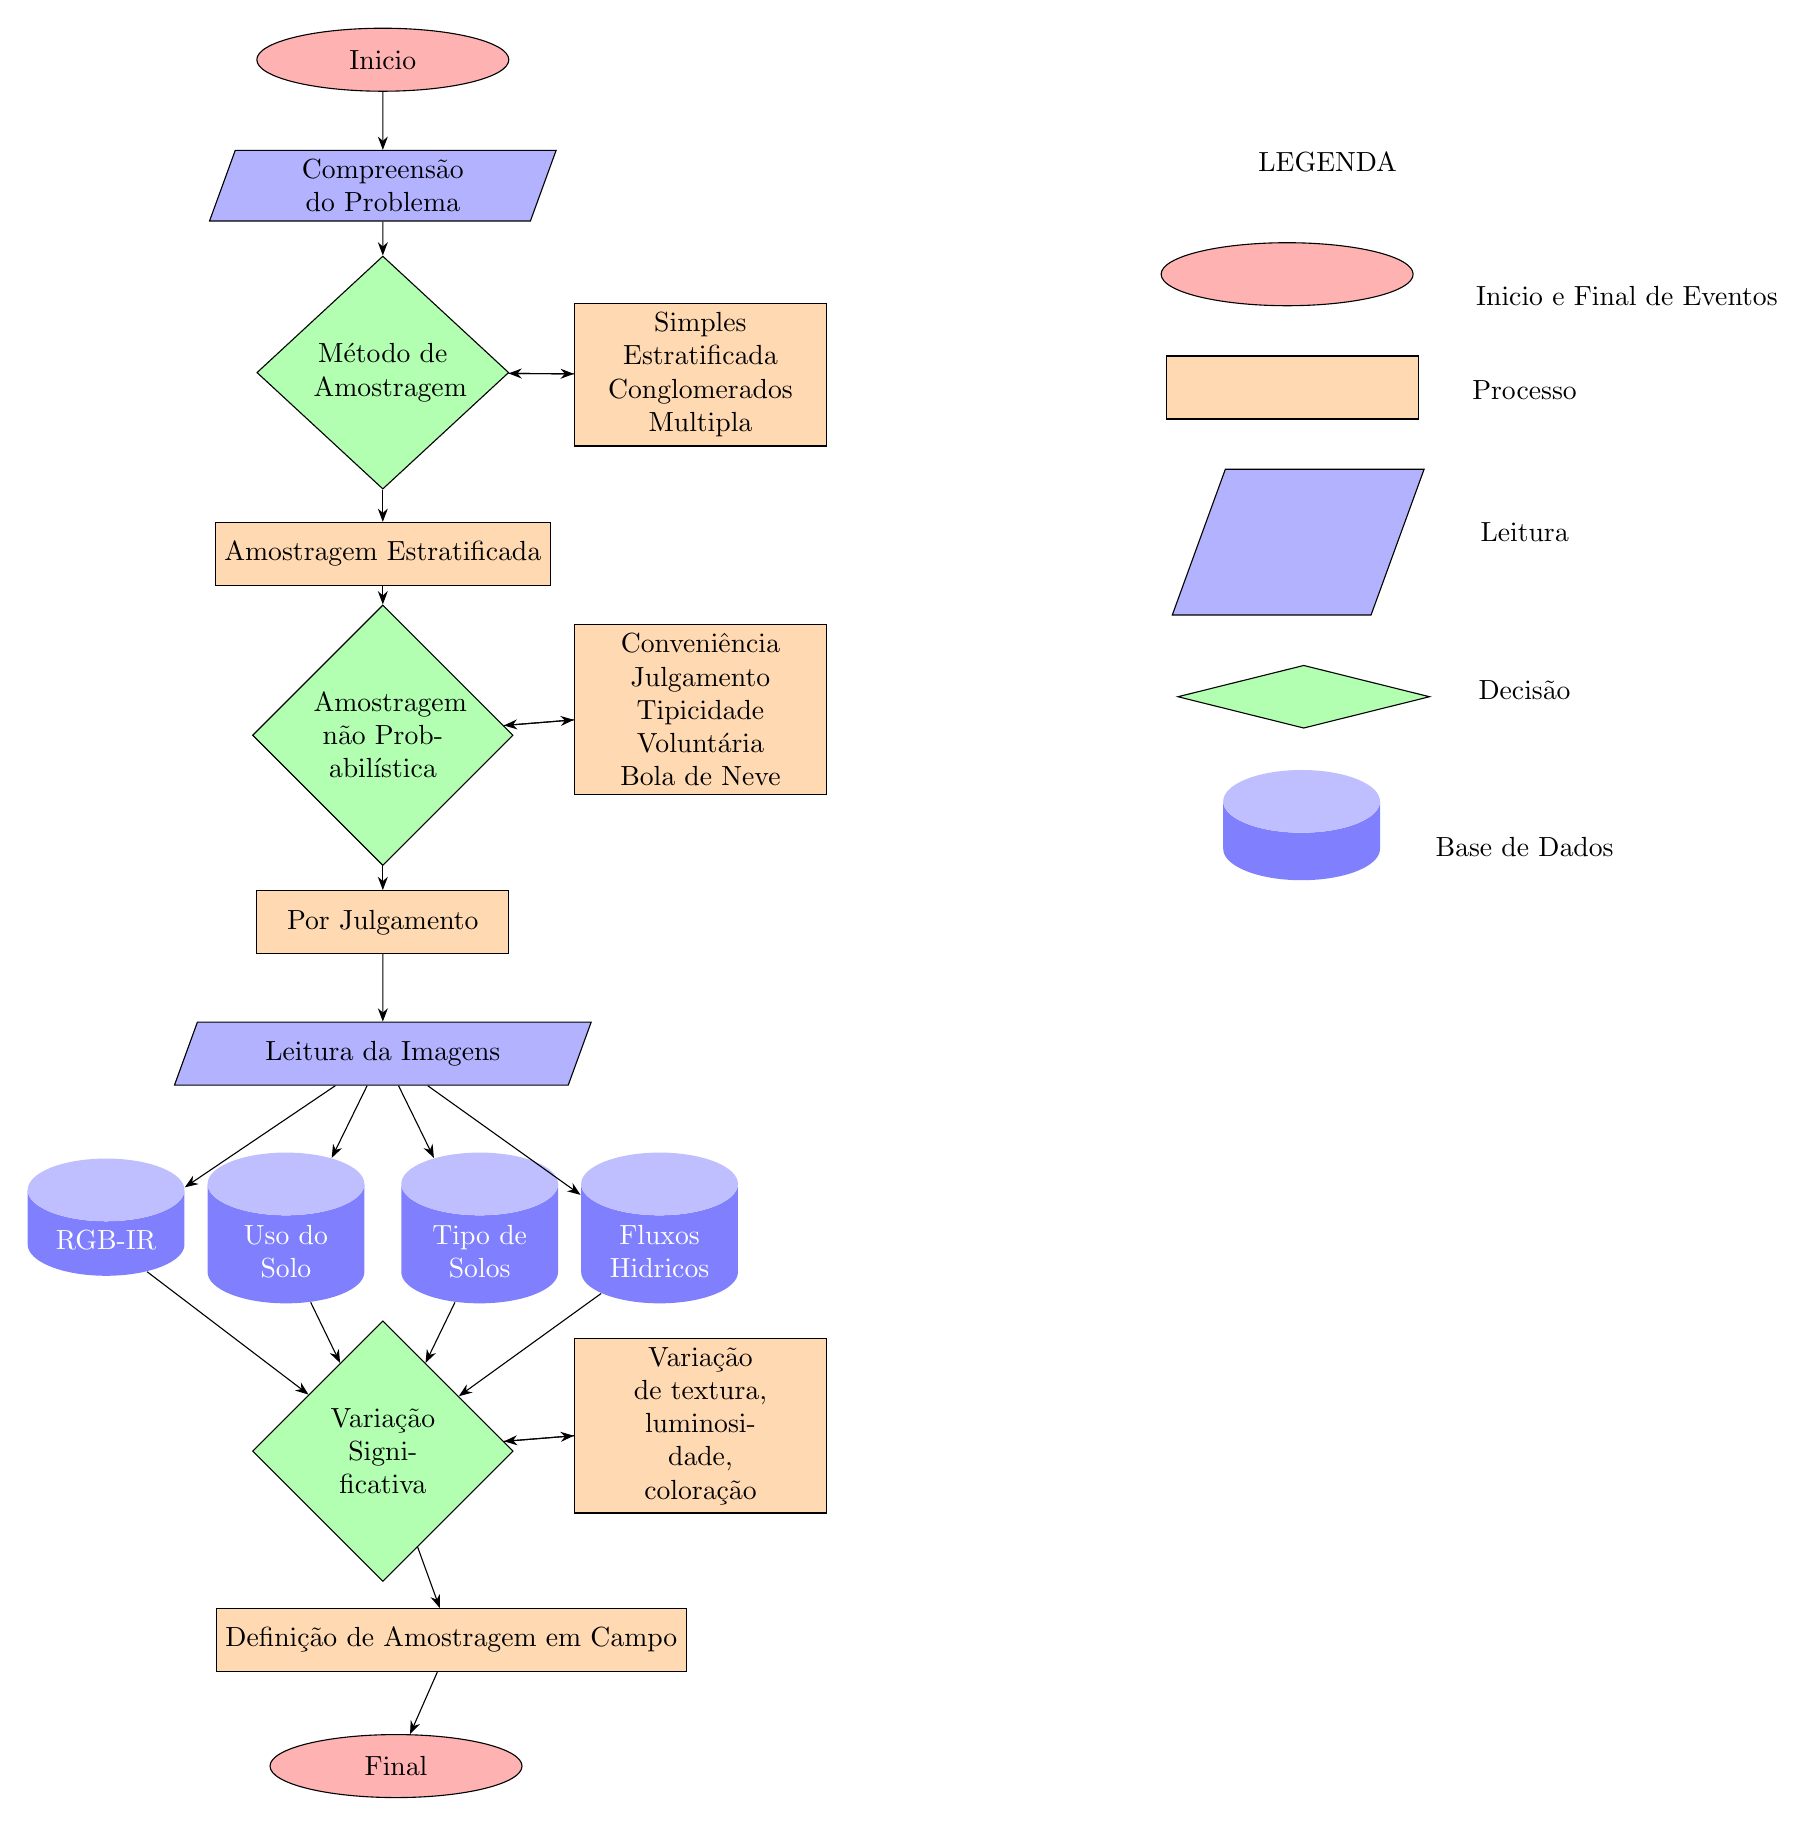
\begin{tikzpicture}[
    node distance = 8mm and 16mm,
      start chain = A going below,
      base/.style = {draw, minimum width=32mm, minimum height=8mm, align=center, on chain=A},
 startstop/.style = {base, ellipse, rounded corners, fill=red!30},
   process/.style = {base, rectangle, fill=orange!30},
        io/.style = {base, trapezium, 
                     trapezium left angle=70, trapezium right angle=110,
                     fill=blue!30},
  decision/.style = {base, diamond, fill=green!30},
  every edge quotes/.style = {auto=right}]
                    ]
  \node [startstop]  (start) {Inicio};
  \node [io, below of=start, text width=10em] (leitura0)   {Compreensão do Problema};   
  \node [decision, below of=leitura0, text width=5em, yshift =-2.2em](decisao1)   { Método de Amostragem };
   \node [process, right of=decisao1, xshift =+9.2em, yshift =+2.2em]  (tipos1){ Simples \\ Estratificada \\ Conglomerados \\ Multipla   };   
  \node [process, below of=decisao1, xshift =-0.0em, yshift =-2.0em](escolha)  {Amostragem Estratificada};   
   \node [decision, below of=escolha, text width=5em, xshift =-0.0em, yshift =-2.0em] (decisao2)  {Amostragem não Probabilística}; 
    \node [process, right of=decisao2, xshift =+9.2em, yshift = +3.2em] (Alternaticas2)        {Conveniência \\ Julgamento \\ Tipicidade \\ Voluntária \\ Bola de Neve};
   \node [process, below of=decisao2, xshift =-0.0em, yshift =-2.2em]  (julgamento1)       {Por Julgamento};
    % 
     \node [io, below of=julgamento1, yshift =-0.2em ] (leitura2)             {Leitura da Imagens};
    %
     \node[cylinder, below of=leitura2, cylinder uses custom fill, cylinder end fill=blue!25,   cylinder body fill=blue!50,shape border rotate=90,text=white,  aspect=0.4,minimum width=1cm,minimum height=1.4cm, below of=leitura2,  text width=5em,align=center,xshift=-10.0em, yshift =-2.2em ](Store1){RGB-IR}; % Imagens RGB 
    %
     \node[cylinder, below of=leitura2,  cylinder uses custom fill, cylinder end fill=blue!25,   cylinder body fill=blue!50,shape border rotate=90,text=white,  aspect=0.4,minimum width=1cm,minimum height=1.4cm, below of=decisao1,  text width=5em,align=center,xshift=-3.5em, yshift =-27.2em ](Store2){Uso do Solo}; %Uso do Solo
    %---
     \node[cylinder, below of=leitura2,  cylinder uses custom fill, cylinder end fill=blue!25,   cylinder body fill=blue!50,shape border rotate=90,text=white,  aspect=0.4,minimum width=1cm,minimum height=1.4cm, below of=decisao1,  text width=5em,align=center,xshift=+3.5em, yshift =-27.2em  ](Store3){Tipo  de Solos}; %Tipo de solos
    %%
    \node[cylinder, below of=leitura2,  cylinder uses custom fill, cylinder end fill=blue!25,   cylinder body fill=blue!50,shape border rotate=90,text=white,  aspect=0.4,minimum width=1cm,minimum height=1.4cm, below of=decisao1,  text width=5em,align=center,xshift=+10.0em, yshift =-27.2em  ](Store4){Fluxos   Hidricos}; %Tipo de solos
    %===
    \node [decision,  text width=5em, yshift =-6.2em ] (variac1)       { Variação Significativa};
    %===
     \node [process, right of=variac1,  text width=5em, xshift =+9.2em , yshift =+3.2em ]  (variacao)       {Variação de textura, luminosidade, coloração};
    %----
    \node [process, below of=variacao, xshift =-9.0em, yshift =-3.2em ] (defin)        {Definição de Amostragem em Campo};
    \node [startstop, below of=defin, xshift =-2.0em]  (final) { Final};
    %---
    \draw [arrows=-Stealth] 
      (start) edge[" "]  (leitura0)
      (leitura0) edge[" "]  (decisao1) 
        (decisao1) edge[" "]  (tipos1)
        (tipos1) edge[" "]   (decisao1) 
      (decisao1)  edge[" "] (escolha) 
      (escolha)   edge[" "] (decisao2)
     (decisao2)edge[" "]  (Alternaticas2) 
       (Alternaticas2)edge[" "]  (decisao2)
      (decisao2) edge[" "]  (julgamento1) 
       (julgamento1) edge[" "]   (leitura2)  
        (leitura2)  edge[" "]   (Store1)
         (leitura2)  edge[" "]   (Store2)
         (leitura2)  edge[" "]   (Store3)
         (leitura2)  edge[" "]   (Store4)
         (Store4) edge[" "]   (variac1) 
          (Store3)edge[" "]   (variac1) 
           (Store2)edge[" "]   (variac1) 
            (Store1)edge[" "]   (variac1)
            (variac1)edge[" "]   (variacao) 
           (variacao)  edge[" "]  (variac1) 
            (variac1)  edge[" "]  (defin) 
            (defin) edge[" "] (final) 
    ;
    %%%%%%
      \node at (12, -1.3)  {LEGENDA} ;
    \node [startstop,xshift =+32.2em, yshift =+58.5em  ]  { };
    \node at (15.8, -3.0)  {Inicio e Final de Eventos} ;
    \node [process,xshift =+0.2em, yshift =+0.5em  ]   { };
    \node at (14.5, -4.2)  {Processo} ;
    \node [io, xshift =+0.2em, yshift =+0.5em  ]   { };
    \node at (14.5, -6.0)  {Leitura} ;
    \node [decision,xshift =+0.2em, yshift =+0.5em  ]   { };
    \node at (14.5, -8.0)  {Decisão} ;
   \node[cylinder, cylinder uses custom fill, cylinder end fill=blue!25,   cylinder body fill=blue!50,shape border rotate=90,text=white,  aspect=0.4,minimum width=1cm,minimum height=1.4cm ,  text width=5em,align=center,xshift =+33.2em, yshift =-28.5 em  ] { }; 
    \node at (14.5, -10.0)  {Base de Dados} ;
    %
    %%%%%%   %% 
  \end{tikzpicture}
  
   \begin{comment}
  	
 
  	\begin{figure}
  		\centering
  		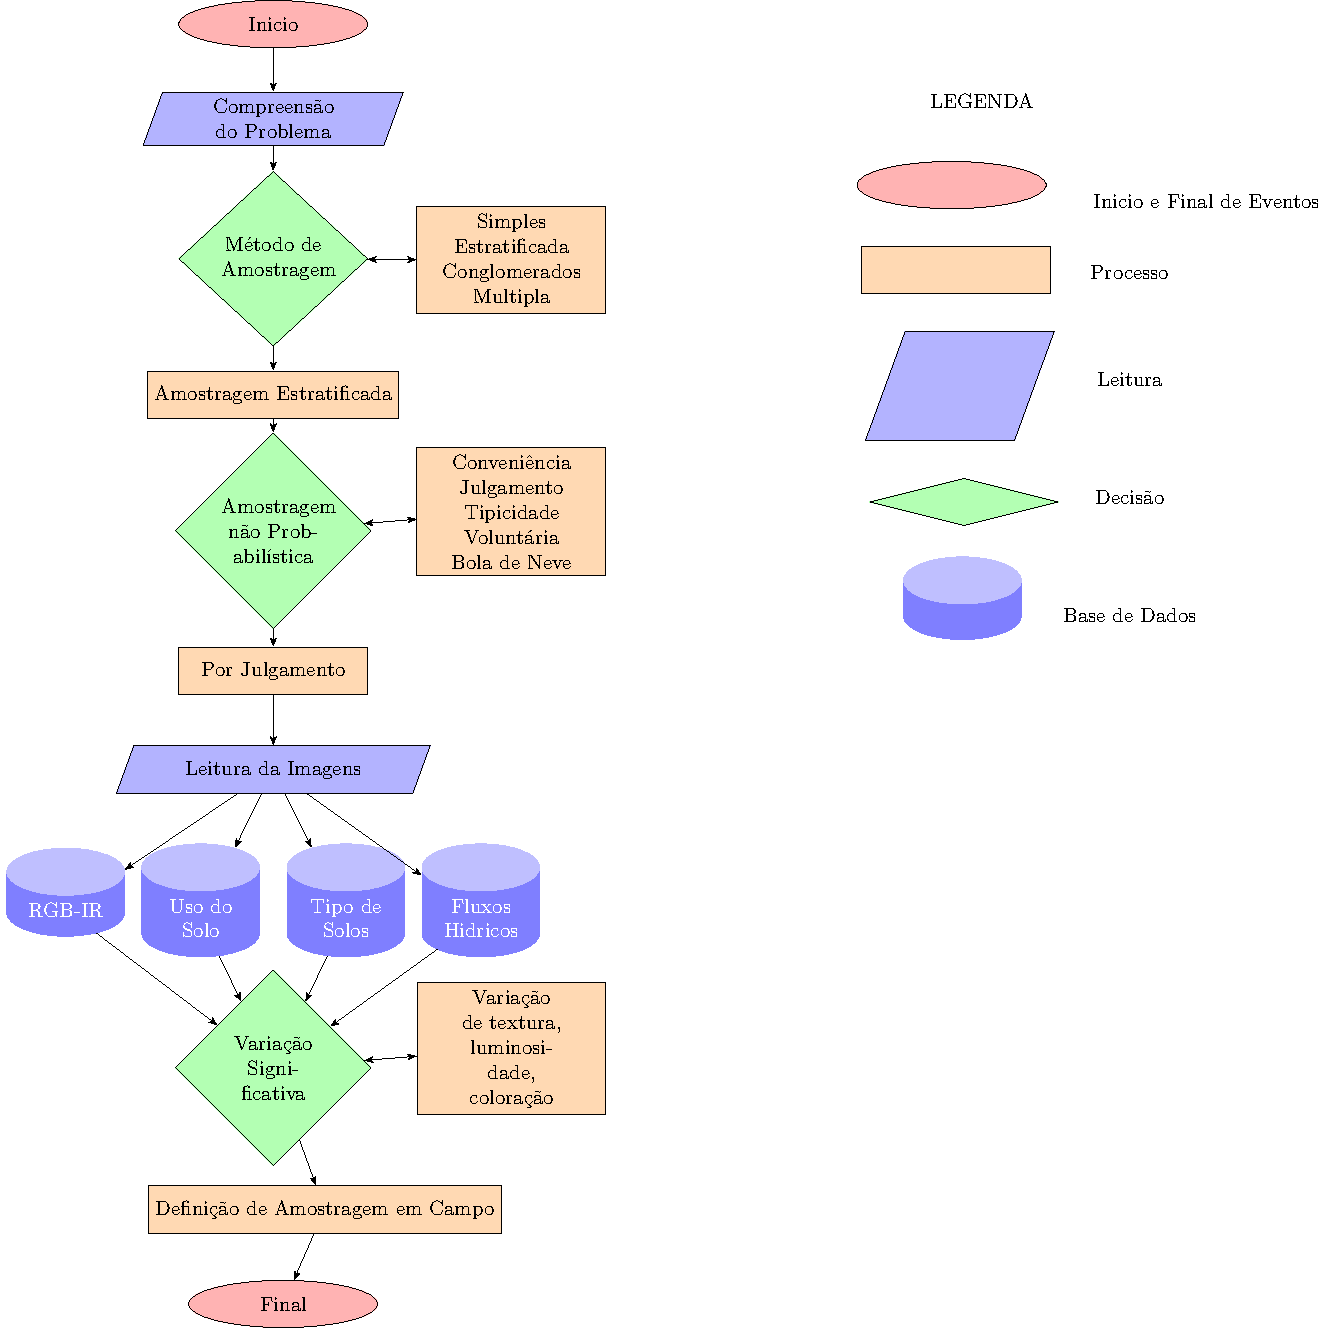
\includegraphics[width=0.97\linewidth]{DIAGRAMAS/flow-diagrama-Alterado2}
  		\caption{\href{file:./DIAGRAMAS/flow-diagrama-Alterado2.tex}{TEX File} }
  		\label{fig:flow-diagrama-Alterado2}
  	\end{figure}
  	
  \end{comment}	
  
  
\end{document}